
\documentclass[reqno, UTF8]{amsart}
%Typical documenttypes: article/book
%some examples:
%\documentclass[reqno,11pt]{book}   %%%for books
%\documentclass[]{minimal}			%%%for Minimal Working Example


%for beamers, you have to change a lot. Especially, remove the package enumitem!!!



%%%%%%%%%%%%%%%%%%%% setting for fast compiling

%\special{dvipdfmx:config z 0}		% no compression

%\includeonly{chapters/chapter9}		% In practice, use an empty document called "chapter9"	% usually for printing books






%%%%%%%%%%%%%%%%%%%% here we include packages

%%%basic packages for math articles
\usepackage{amssymb}
\usepackage{amsthm}
\usepackage{amsmath}
\usepackage{amsfonts}
\usepackage[shortlabels]{enumitem}	% It supersedes both enumerate and mdwlist. The package option shortlabels is included to configure the labels like in enumerate.

%%%packages for special symbols
\usepackage{pifont}					% Access to PostScript standard Symbol and Dingbats fonts
\usepackage{wasysym}				% additional characters
\usepackage{bm}						% bold fonts: \bm{...}
\usepackage{extarrows}				% may be replaced by tikz-cd
%\usepackage{unicode-math}			% unicode maths for math fonts, now I don't know how to include it
%\usepackage{ctex}					% Chinese characters, huge difference.


%%%basic packages for fancy electronic documents
\usepackage[colorlinks]{hyperref}
\usepackage[table,hyperref]{xcolor} 			% before tikz-cd. 
%\usepackage[table,hyperref,monochrome]{xcolor}	% disable colored output (black and white)

%%%packages for figures and tables (general setting)
\usepackage{float}				%Improved interface for floating objects
\usepackage{caption,subcaption}
\usepackage{adjustbox}			% for me it is usually used in tables 
\usepackage{stackengine}		%baseline changes

%%%packages for commutative diagrams
\usepackage{tikz-cd}
\usepackage{quiver}			% see https://q.uiver.app/

%%%packages for pictures
\usepackage[width=0.5,tiewidth=0.7]{strands}
\usepackage{graphicx}			% Enhanced support for graphics

%%%packages for tables and general settings
\usepackage{array}
\usepackage{makecell}
\usepackage{multicol}
\usepackage{multirow}
\usepackage{diagbox}
\usepackage{longtable}

%%%packages for ToC, LoF and LoT







 %https://tex.stackexchange.com/questions/58852/possible-incompatibility-with-enumitem








%%%%%%%%%%%%%%%%%%%% here we include theoremstyles

\numberwithin{equation}{section}

\theoremstyle{plain}
\newtheorem{theorem}{Theorem}[section]

\newtheorem{setting}[theorem]{Setting}
\newtheorem{definition}[theorem]{Definition}
\newtheorem{lemma}[theorem]{Lemma}
\newtheorem{proposition}[theorem]{Proposition}
\newtheorem{corollary}[theorem]{Corollary}
\newtheorem{conjecture}[theorem]{Conjecture}

\newtheorem{claim}[theorem]{Claim}
\newtheorem{eg}[theorem]{Example}
\newtheorem{ex}[theorem]{Exercise}
\newtheorem{fact}[theorem]{Fact}
\newtheorem{ques}[theorem]{Question}
\newtheorem{answ}[theorem]{Answer}
\newtheorem{warning}[theorem]{Warning}
\newtheorem{notation}[theorem]{Notations}


\newtheorem*{bbox}{Black box}



\numberwithin{equation}{section}


\theoremstyle{remark}

\newtheorem{remark}[theorem]{Remark}
\newtheorem*{remarks}{Remarks}
\newenvironment{proofsketch}
  {\begin{proof}[Sketch of proof]}
  {\end{proof}}
%%% for important theorems
%\newtheoremstyle{theoremletter}{4mm}{1mm}{\itshape}{ }{\bfseries}{}{ }{}
%\theoremstyle{theoremletter}
%\newtheorem{theoremA}{Theorem}
%\renewcommand{\thetheoremA}{A}
%\newtheorem{theoremB}{Theorem}
%\renewcommand{\thetheoremB}{B}







%%%%%%%%%%%%%%%%%%%% here we declare some symbols

%%%%%%%DeclareMathOperator
%see here for why newcommand is better for DeclareMathOperator: https://tex.stackexchange.com/questions/67506/newcommand-vs-declaremathoperator

%%%%%basic symbols. Keep them!

%%%symbols for sets and maps
\DeclareMathOperator{\pt}{\operatorname{pt}}	%points. Other possibilities are \{pt\}, \{*\}, pt, * ...
\DeclareMathOperator{\Id}{\operatorname{Id}}	%identity in groups.
\DeclareMathOperator{\Img}{\operatorname{Im}}

\DeclareMathOperator{\Ob}{\operatorname{Ob}}
\DeclareMathOperator{\Mor}{\operatorname{Mor}}	%difference of Mor and Hom: Hom is usually for abelian categories
\DeclareMathOperator{\Hom}{\operatorname{Hom}}	\DeclareMathOperator{\End}{\operatorname{End}}
\DeclareMathOperator{\Aut}{\operatorname{Aut}}

%%%symbols for linear algebras and 
%%linear algebras
\DeclareMathOperator{\tr}{\operatorname{tr}}
\DeclareMathOperator{\diag}{\operatorname{diag}}	%for diagonal matrices

%%abstract algebras
\DeclareMathOperator{\ord}{\operatorname{ord}}
\DeclareMathOperator{\gr}{\operatorname{gr}}
\DeclareMathOperator{\Frac}{\operatorname{Frac}}

%%%symbols for basic geometries
\DeclareMathOperator{\vol}{\operatorname{vol}}	%volume
\DeclareMathOperator{\dist}{\operatorname{dist}}
\DeclareMathOperator{\supp}{\operatorname{supp}}

%%%symbols for category
%%names of categories
\DeclareMathOperator{\Mod}{\operatorname{Mod}}
\DeclareMathOperator{\Vect}{\operatorname{Vect}}


%%%symbols for homological algebras
\DeclareMathOperator{\Tor}{\operatorname{Tor}}
\DeclareMathOperator{\Ext}{\operatorname{Ext}}
\DeclareMathOperator{\gldim}{\operatorname{gl.dim}}
\DeclareMathOperator{\projdim}{\operatorname{proj.dim}}
\DeclareMathOperator{\injdim}{\operatorname{inj.dim}}
\DeclareMathOperator{\rad}{\operatorname{rad}}


%%%symbols for algebraic groups
\DeclareMathOperator{\GL}{\operatorname{GL}}
\DeclareMathOperator{\SL}{\operatorname{SL}}

%%%symbols for typical varieties
\DeclareMathOperator{\Gr}{\operatorname{Gr}}
\DeclareMathOperator{\Flag}{\operatorname{Flag}}

%%%symbols for basic algebraic geometry
\DeclareMathOperator{\Spec}{\operatorname{Spec}}
\DeclareMathOperator{\Coh}{\operatorname{Coh}}
\newcommand{\Dcoh}{\mathcal{D}_{\operatorname{Coh}}}%%%This one shows the difference between \DeclareMathOperator and \newcommand
\DeclareMathOperator{\Pic}{\operatorname{Pic}}
\DeclareMathOperator{\Jac}{\operatorname{Jac}}

%%%%%advanced symbols. Choose the part you need!

%%%symbols for algebraic representation theory
\DeclareMathOperator{\ind}{\operatorname{ind}}	%\ind(Q) means the set of  equivalence classes of finite dimensional indecomposable representations
\DeclareMathOperator{\Res}{\operatorname{Res}}
\DeclareMathOperator{\Ind}{\operatorname{Ind}}
\DeclareMathOperator{\cInd}{\operatorname{c-Ind}}


\DeclareMathOperator{\Rep}{\operatorname{Rep}}
\DeclareMathOperator{\rep}{\operatorname{rep}} %usually rep means the category of finite dimensional representations, while Rep means the category of representations.
\DeclareMathOperator{\Irr}{\operatorname{Irr}}
\DeclareMathOperator{\irr}{\operatorname{irr}}
\DeclareMathOperator{\Adm}{\operatorname{\Pi}}
\DeclareMathOperator{\Char}{\operatorname{Char}}
\DeclareMathOperator{\WDrep}{\operatorname{WDrep}}

%%%symbols for algebraic topology
\DeclareMathOperator{\EGG}{\operatorname{E}\!}
\DeclareMathOperator{\BGG}{\operatorname{B}\!}

\DeclareMathOperator{\chern}{\operatorname{ch}^{*}}
\DeclareMathOperator{\Td}{\operatorname{Td}}
\DeclareMathOperator{\AS}{\operatorname{AS}}	%Atiyah--Segal completion theorem 

%%%symbols for Auslander--Reiten theory 
\DeclareMathOperator{\Modup}{\overline{\operatorname{mod}}}
\DeclareMathOperator{\Moddown}{\underline{\operatorname{mod}}}
\DeclareMathOperator{\Homup}{\overline{\operatorname{Hom}}}
\DeclareMathOperator{\Homdown}{\underline{\operatorname{Hom}}}


%%%symbols for operad
\DeclareMathOperator{\Com}{\operatorname{\mathcal{C}om}}
\DeclareMathOperator{\Ass}{\operatorname{\mathcal{A}ss}}
\DeclareMathOperator{\Lie}{\operatorname{\mathcal{L}ie}}
\DeclareMathOperator{\calEnd}{\operatorname{\mathcal{E}nd}} %cal=\mathcal


%%%%%personal symbols. Use at your own risk!

%%%symbols only for master thesis
\DeclareMathOperator{\ptt}{\operatorname{par}}	%the partition map
\DeclareMathOperator{\str}{\operatorname{str}}	%strict case
\DeclareMathOperator{\RRep}{\widetilde{\operatorname{Rep}}}
\DeclareMathOperator{\Rpt}{\operatorname{R}}
\DeclareMathOperator{\Rptc}{\operatorname{\mathcal{R}}}
\DeclareMathOperator{\Spt}{\operatorname{S}}
\DeclareMathOperator{\Sptc}{\operatorname{\mathcal{S}}}
\DeclareMathOperator{\Kcurl}{\operatorname{\mathcal{K}}}
\DeclareMathOperator{\Hcurl}{\operatorname{\mathcal{H}}}
\DeclareMathOperator{\eu}{\operatorname{eu}}
\DeclareMathOperator{\Eu}{\operatorname{Eu}}
\DeclareMathOperator{\dimv}{\operatorname{\underline{\mathbf{dim}}}}
\DeclareMathOperator{\St}{\mathcal{Z}}

%%%%%symbols which haven't been classified. Add your own math operators here!

\DeclareMathOperator{\Perv}{\operatorname{Perv}}
\DeclareMathOperator{\Alb}{\operatorname{Alb}}
\DeclareMathOperator{\Sp}{\operatorname{Sp}}
\DeclareMathOperator{\SO}{\operatorname{SO}}
\DeclareMathOperator{\E6}{\operatorname{E}_6}
\DeclareMathOperator{\cc}{\operatorname{cc}}
\DeclareMathOperator{\Hnm}{\operatorname{H}}
\DeclareMathOperator{\-mod}{\!\operatorname{-mod}}
\DeclareMathOperator{\divisor}{\operatorname{div}}
\DeclareMathOperator{\rank}{\operatorname{rank}}
\DeclareMathOperator{\CH}{\operatorname{CH}}
\DeclareMathOperator{\sign}{\operatorname{sign}}
\DeclareMathOperator{\longleftmapsto}{\rotatebox[origin=c]{180}{$\;\longmapsto\;$}}
\DeclareMathOperator{\Zsm}{Z^{\operatorname{sm}}}
\DeclareMathOperator{\Gal}{\operatorname{Gal}}
\DeclareMathOperator{\Mon}{\operatorname{Mon}}
\DeclareMathOperator{\AJ}{\operatorname{AJ}}
\DeclareMathOperator{\AP}{\operatorname{AP}}
\newcommand{\covermap}{h}
\DeclareMathOperator{\Prym}{\operatorname{Prym}}
\DeclareMathOperator{\Nm}{\operatorname{Nm}}
\DeclareMathOperator{\gon}{\operatorname{gon}}
\DeclareMathOperator{\univ}{\operatorname{univ}}
\DeclareMathOperator{\Abel}{\operatorname{Abel}}
\DeclareMathOperator{\pr}{\operatorname{pr}}
\DeclareMathOperator{\aff}{\operatorname{aff}}

%%%%%%%newcommand

%%%basic symbols
\newcommand{\norm}[1]{\Vert{#1}\Vert}





%%%%%%%%%%%%%%%%%%%% here we make some blocks for special features. 

%%%% todo notes %%%%
\usepackage[colorinlistoftodos,textsize=footnotesize]{todonotes}
\setlength{\marginparwidth}{2.5cm}
\newcommand{\leftnote}[1]{\reversemarginpar\marginnote{\footnotesize #1}}
\newcommand{\rightnote}[1]{\normalmarginpar\marginnote{\footnotesize #1}\reversemarginpar}









%%%%%%%%%%%%%%%%%%%% here we make some global settings. Understand everything here before you make a document!

\usepackage[a4paper,left=3cm,right=3cm,bottom=4cm]{geometry}
\usepackage{indentfirst}	% Indent first paragraph after section header

\setcounter{tocdepth}{1}


%https://latexref.xyz/_005cparindent-_0026-_005cparskip.html
\setlength{\parindent}{15pt}	
\setlength{\parskip}{0pt plus1.5pt}

%\setlength\intextsep{0cm}
%\setlength\textfloatsep{0cm}
\def\arraystretch{1}
%\setcounter{secnumdepth}{3}

\allowdisplaybreaks


\begin{document}

% The beginning depends on the documentclass. Rewrite this part if you use different documentclass!
\date{\today}

\title
{Subvarieties in complex abelian varieties 
}
\author{Xiaoxiang Zhou}
\address{Institut für Mathematik\\
Humboldt-Universität zu Berlin\\
Berlin, 12489\\ Germany\\} 
\email{email:xiaoxiang.zhou@hu-berlin.de}


\maketitle
\tableofcontents

\section{Introduction}
From any subvariety of an abelian variety one obtains a reductive group via the convolution of perverse sheaves; in this way, traditional questions in algebraic geometry can be reinterpreted in representation-theoretic terms, providing new geometric perspectives.

In \cite{Kr20}, Prof. Krämer shows that Weyl group orbits correspond to conic Lagrangian cycles in the cotangent bundle, which are realized as the conormal bundles of certain subvarieties. A careful analysis of these subvarieties is frequently central to resolving the problems at hand, cf. \cite[\S 5-\S 8]{JKLM22}. Here we investigate three principal properties of these subvarieties: irreducibility, dimension, and homology class.

Concerning irreducibility, we observe that the irreducible components correspond precisely to the orbits of the monodromy group. Hence, the discrepancy between the monodromy group and the Weyl group provides a measure of the failure of irreducibility of these subvarieties. Recently, we constructed an example where the monodromy group is significantly smaller than expected, thereby disproving \cite[Conjecture~8]{Kr16cubicthreefold}:

\begin{proposition}\label{prop: smallmongp}
There exists an étale double cover $h: C \to C'$ of smooth projective curves such that the Abel--Prym map
$\AP_{C/C'}: C \longrightarrow A$
is an embedding, and 
\begin{equation*}
\begin{aligned}
  W_C\cong\;& S_2^{\oplus d/2} \rtimes S_{d/2}  \\ 
   M_C\subseteq\;& S_4^{\oplus d/4} \rtimes S_{d/4}  \\ 
\end{aligned}
\end{equation*}
where $d = 2g(C')-2$, and $W_C$, $M_C$ denote the Weyl and monodromy groups, respectively.
\end{proposition}
This turns out to be the only nontrivial example in the Prym setting when $g(C') > 9$.

For the dimension and homology class of a subvariety $Z$, both invariants can be recovered from the homology class of $\mathbb{P}\Lambda_{Z} \subset \mathbb{P}T^*A$ — that is, from the Chern--Mather class of $Z$. Standard computational techniques are available when the group is a full or signed symmetric group. This applies in particular to the Jacobian case, which will be analyzed in detail in Section ???.

\section*{Acknowledgement}
%\addcontentsline{toc}{section}{Acknowledgement}

I would like to express my sincere gratitude to my supervisor, Thomas Krämer, without whose support this work would not have been possible. He proposed the problem, guided me throughout the project, and generously spent many hours discussing drafts and explaining important ideas. I am also thankful to Haohao Liu, Chenji Fu, Zhixing Chen, Vincent Ariksoy, Aaron Beumer, Roben de Preter, Andreas Kretschmer, Andrés Rojas, Søren Gammelgaard, Paweł Borówka, and Gavril Farkas for their insightful discussions and valuable comments. Funding is provided by the Deutsche Forschungsgemeinschaft (DFG, German Research Foundation) under Germany´s Excellence Strategy – The Berlin Mathematics Research Center MATH+ (EXC-2046/1, project ID: 390685689).
%%%%%%%%%%%%%%%%%%%%%%%%%%%%%%%%%%%%%%%%%%%%%%%%%%%%
\section{Tangent Gauss map and conormal Gauss map}
For simplicity, we work over the base field $\kappa = \mathbb{C}$, and by a variety we mean a integral separated scheme of finite type over $\mathbb{C}$. Let $A/\mathbb{C}$ be an abelian variety of dimension $n$, and let $Z \subseteq A$ be an irreducible closed subvariety of dimension $r$. We denote by $\iota_Z: Z \hookrightarrow A$ the inclusion morphism.\footnote{I'm not sure whether we should consider the more general cases in the future—such as working over a field of characteristic $p$, letting $A$ be a semiabelian variety or a complex torus, or allowing $\iota$ to be a covering onto its image. For now, I will omit these possibilities from this document.}

\subsection{Gauss map and monodromy group}
\begin{definition}
For a subvariety $Z \subset A$, the tangent Gauss map of $Z$ is defined as 
$$\phi_Z: \Zsm \longrightarrow \Gr(r,T_0 A) \qquad p \longmapsto T_pZ \;\;\subseteq T_pA \cong T_0 A$$
which describes the tangent space information at each point.
\end{definition} 

\begin{remark}
Any map $X\longrightarrow\Gr(r, V)$ is induced by a rank $r$ vector bundle $\mathcal{E}$ on $X$ together with an epimorphism $V^{*}\otimes \mathcal{O}_X \twoheadrightarrow \mathcal{E}$. In our case, the map $\phi_Z$ is induced by the tangent bundle $\mathcal{T}_{\Zsm}$ and the sections
$$T_0^{*} A \otimes_{\mathbb{C}} \mathcal{O}_{\Zsm} \subseteq\Hnm^0(\Zsm,\mathcal{T}_{\Zsm}^{\vee}) \otimes_{\mathbb{C}} \mathcal{O}_{\Zsm} \twoheadrightarrow \mathcal{T}_{\Zsm}^{\vee}.$$
\end{remark}


The definition of the conormal Gauss map requires a brief recollection of the conormal variety. On the smooth locus, the normal and conormal bundles behave well as vector bundles:\footnote{This is more symmetric when writing them as short exact sequences:
% https://q.uiver.app/#q=WzAsMTAsWzMsMCwiXFxtYXRoY2Fse059X3tcXFpzbS9BfSJdLFsxLDAsIlxcbWF0aGNhbHtUfV97XFxac219Il0sWzIsMCwiXFxtYXRoY2Fse1R9X0F8X3tcXFpzbX0iXSxbMSwxLCJcXExhbWJkYV97XFxac219ICJdLFsyLDEsIlxcT21lZ2FfQXxfe1xcWnNtfSAiXSxbMywxLCJcXE9tZWdhX3tcXFpzbX0gIl0sWzQsMCwiMCJdLFs0LDEsIjAiXSxbMCwwLCIwIl0sWzAsMSwiMCJdLFsxLDJdLFsyLDBdLFszLDRdLFs0LDVdLFswLDZdLFs1LDddLFs4LDFdLFs5LDNdXQ==
\[\begin{tikzcd}[ampersand replacement=\&,column sep=2.25em,row sep=tiny]
	0 \& {\mathcal{T}_{\Zsm}} \& {\mathcal{T}_A|_{\Zsm}} \& {\mathcal{N}_{\Zsm/A}} \& 0 \\
	0 \& {\mathcal{N}_{\Zsm/A}^* } \& {\Omega_A|_{\Zsm} } \& {\Omega_{\Zsm} } \& 0
	\arrow[from=1-1, to=1-2]
	\arrow[from=1-2, to=1-3]
	\arrow[from=1-3, to=1-4]
	\arrow[from=1-4, to=1-5]
	\arrow[from=2-1, to=2-2]
	\arrow[from=2-2, to=2-3]
	\arrow[from=2-3, to=2-4]
	\arrow[from=2-4, to=2-5]
\end{tikzcd}\]
}
$$\mathcal{N}_{\Zsm/A} := \mathcal{T}_A|_{\Zsm} \;/\; \mathcal{T}_{\Zsm} \qquad \mathcal{N}_{\Zsm/A}^* = \ker \left( \Omega_A|_{\Zsm} \rightarrow \rule{0mm}{3.4mm} \Omega_{\Zsm} \right).$$
We write $\Lambda_{\Zsm}$ as the total space of $\mathcal{N}_{\Zsm/A}^*$.
The conormal variety $\Lambda_{Z}$ is the closure of $\Lambda_{\Zsm}$ viewed as a subvariety in $T^*A$:
$$\Lambda_{Z}:=\;\; \overline{\Lambda_{\Zsm}} \;\; \subset T^*A \;\cong\; A \times T^{*}_{0}A$$
this is a conical Lagrangian cycle in $T^*A$. The (affine) conormal Gauss map is defined as
$$\gamma_Z^{\aff}: \Lambda_{Z} \subset A \times T^{*}_{0}A \longrightarrow T^{*}_{0}A$$

For intersection-theoretic purposes it is more natural to work with projectivized conormal spaces. We therefore pass from the affine conormal Gauss map to its projectivized version:
\begin{definition}
the projectivized conormal variety
$$\mathbb{P}\Lambda_{Z}:=\;\; \overline{\mathbb{P}\Lambda_{\Zsm}} \;\; \subset \mathbb{P}T^*A \;\cong\; A \times \mathbb{P}T^{*}_{0}A$$
is a Legendrian cycle in the contact variety $A \times \mathbb{P}T^{*}_{0}A$. $\mathbb{P}\Lambda_{\Zsm}$ is a $\mathbb{P}^{r-1}$-bundle over $\Zsm$, and the map 
$$\gamma_Z: \mathbb{P}\Lambda_{Z} \subset A \times \mathbb{P}T^{*}_{0}A \longrightarrow \mathbb{P}T^{*}_{0}A$$
is called the (projectivized) conormal Gauss map.
\end{definition} 
By \cite[Theorem 2.8 (1)]{JKLM22}, $\gamma_Z$ is generically finite when $Z$ is (an integral variety) of general type.

A lot of geometry of $Z$ is encoded in the map $\gamma_Z$. For instance, if $Z \subset A$ is smooth, then 
$$\deg \gamma_Z = (-1)^r \chi(Z),$$
where $\chi(Z)=\sum_i (-1)^i b_i(Z)$ is the topological Euler characteristic of $Z$.

Further insight can be gained by analyzing the fibers of $\gamma_Z$. For instance, if $Z$ is preserved by a translation $t_v: A\longrightarrow A$, then each fiber $\gamma_Z^{-1}(\xi)$ is also invariant under $t_v$. Likewise, if $Z = -Z$, then the fiber satisfies $\gamma_Z^{-1}(\xi) = -\gamma_Z^{-1}(\xi)$. Finding further constraints is more challenging.\footnote{You can imagine the fiber $\gamma_Z^{-1}(\xi)$ as a cluster of stars projected onto a celestial dome. As $\xi$ varies, these points shift, tracing out paths much like stars drifting across the night sky. The constraints that govern them are subtle, like the imagined lines that shape constellations. And in the long arc of variation, monodromy emerges—like the slow turning that replaces Kochab with Polaris among the stars.}

An important invariant arising from the fiber $\gamma_Z^{-1}(\xi)$ is the monodromy group $\Gal(\gamma_Z)$; for completeness, we recall its definition below.

\begin{definition}
Let $f: Y \to X$ be a generically finite morphism between algebraic varieties. Then there exists a non-empty open subset $U \subseteq X$ such that the restriction $f^{-1}(U) \to U$ is a finite étale cover.
Moving along a closed loop in $U$ induces a permutation of the points in the fiber $f^{-1}(\xi_0)$, which defines the map\footnote{In the last isomorphism we implicitly give an order to the fiber $f^{-1}(\xi)$.}
$$\rho_{f}: \pi_1(U, \xi_0) \longrightarrow \Aut (f^{-1}(\xi_0)) \cong S_{\deg f}.$$ 
The monodromy group is then defined as the image of $\rho_{f}$, i.e.,
$$\Gal(f):= \Img \rho_{f}.$$
It is clear that $\Gal(f)$ doesn't depend on the choice of $U$.
\end{definition}


\subsection{Interpolation via hyperplanes}
In this subsection, we reinterpret $\gamma_Z$ using a functorial and more transparent framework. This permits the definition of the conormal Gauss map and its monodromy group for any morphism $\phi: Z \to \Gr(r,n)$ with $\dim Z = r$, and clarifies the relation between the monodromy group and $\deg \phi$.

Since each non-zero conormal vector $\xi  \in T^{*}_{0}A$ determines a hyperplane $H_{\xi} \in \Gr(n-1, T_0A)$, we have the isomorphisms (To simplify notation, we abbreviate $T^{*}_{0}A$ by $W$.)
\begin{equation*}
\begin{aligned}
   \mathbb{P}T^{*}_{0}A \cong\;& \Gr(n-1, T_0A), \\ 
    \mathbb{P}\Lambda_{\Zsm}=\;& \left\{\, (p,\xi)  \in \Zsm \times \mathbb{P}T^{*}_{0}A \;\middle|\; \xi|_{T_pZ}\! \equiv 0 \,\right\}  \\ 
    \cong\;& \left\{\,\rule{0mm}{3.2mm} (p,H)  \in \Zsm \times \Gr(n-1, W) \;\middle|\; \phi_Z(p) \subseteq H \,\right\}  \\ 
    \cong\;& \left(\phi_Z, \Id \right)^{-1} I_{r, n-1},  \\ 
\end{aligned}
\end{equation*}
where 
$$I_{r, n-1}:= \left\{ \rule{0mm}{3.2mm} (V,H)  \in \Gr(r,W) \times \Gr(n-1, W) \;\middle|\; V \subseteq H \,\right\}$$ 
is the incidence variety relating $\Gr(r,W)$ and $\Gr(n-1, W)$. In these terms, 
\begin{equation*}
\begin{aligned}
    \gamma_Z^{-1}(H) \cap \Zsm=\;& \left\{\, p  \in \Zsm  \;\middle|\; \phi_Z(p) \subseteq H \,\right\}  \\ 
    \cong\;& \phi_Z^{-1}\left(\Gr(r\rule{0mm}{3mm},H)\right)  \\ 
\end{aligned}
\end{equation*}
is the collection of points whose tangent spaces lie entirely within $H$.

Geometrically, the monodromy can be described as follows: given a general hyperplane $H \in \mathbb{P}T^{*}_{0}A$, its preimage consists of $d$ points ${ p_1, \ldots, p_d }$. Moving $H$ continuously along a closed loop causes these points to permute, and the monodromy group $\Gal(\gamma_Z)$ consists of all permutations obtained this way. With this formulation, it suffices to consider the Gauss map $\phi_Z$ alone; the inclusion $\iota_Z: Z \to A$ is no longer required for computing the monodromy group.

\begin{definition}\label{def:general_monodromy}
Let $Z$ be an $r$-dimensional variety and $\phi: Z \longrightarrow \Gr(r,n)$ a morphism. The monodromy group $\Mon(\phi)$ is defined as $\Gal(f_{\phi})$, where
$$f_{\phi}: (\phi,\Id)^{-1} I_{r,n-1} \;\subset\; Z \times \Gr(n-1,n) \stackrel{\pi_2}{\longrightarrow} \Gr(n-1,n).$$
\end{definition}
When $\phi$ is not generically injective, the monodromy group is subject to additional constraints, as captured by the next lemma.
\begin{lemma}\label{lem:wreath_product}
Let $\phi: Z \to \Gr(r,n)$ be generically $k$-to-$1$ onto its image. With a suitable ordering of the fibers, the associated monodromy group $\Mon(\phi)$ is contained in a wreath product
$$S_k \wr S_{d/k}:= \left( S_k^{\oplus d/k} \right) \rtimes S_{d/k}. $$
\end{lemma}
\begin{proof}
Consider the diagram below:  
% https://q.uiver.app/#q=WzAsNyxbMCwwLCJcXHBoaToiXSxbMiwwLCJcXEltZyBaIl0sWzEsMCwiWiJdLFszLDAsIlxcR3IocixuKSJdLFszLDEsIlxcR3IocixIKSJdLFsyLDEsIlxce3FfMSxcXGxkb3RzLHFfe2Qva31cXH0iXSxbMSwxLCJcXHtwXzEsXFxsZG90cyxwX2RcXH0iXSxbMiwxLCJrOjEiLDAseyJzdHlsZSI6eyJoZWFkIjp7Im5hbWUiOiJlcGkifX19XSxbMSwzLCIiLDAseyJzdHlsZSI6eyJ0YWlsIjp7Im5hbWUiOiJob29rIiwic2lkZSI6InRvcCJ9fX1dLFs2LDVdLFs1LDRdLFs2LDIsIlxccm90YXRlYm94W29yaWdpbj1jXXs5MH17JFxcc3Vic2V0JH0iLDEseyJzdHlsZSI6eyJib2R5Ijp7Im5hbWUiOiJub25lIn0sImhlYWQiOnsibmFtZSI6Im5vbmUifX19XSxbNSwxLCJcXHJvdGF0ZWJveFtvcmlnaW49Y117OTB9eyRcXHN1YnNldCR9IiwxLHsic3R5bGUiOnsiYm9keSI6eyJuYW1lIjoibm9uZSJ9LCJoZWFkIjp7Im5hbWUiOiJub25lIn19fV0sWzQsMywiXFxyb3RhdGVib3hbb3JpZ2luPWNdezkwfXskXFxzdWJzZXQkfSIsMSx7InN0eWxlIjp7ImJvZHkiOnsibmFtZSI6Im5vbmUifSwiaGVhZCI6eyJuYW1lIjoibm9uZSJ9fX1dXQ==
\[\begin{tikzcd}[ampersand replacement=\&,row sep=small]
	{\phi:} \&[-10mm] Z \& {\Img Z} \& {\Gr(r,n)} \\
	\& {\{p_1,\ldots,p_d\}} \& {\{q_1,\ldots,q_{d/k}\}} \& {\Gr(r,H)}
	\arrow["{k:1}", two heads, from=1-2, to=1-3]
	\arrow[hook, from=1-3, to=1-4]
	\arrow["{\rotatebox[origin=c]{90}{$\subset$}}"{description}, draw=none, from=2-2, to=1-2]
	\arrow[from=2-2, to=2-3]
	\arrow["{\rotatebox[origin=c]{90}{$\subset$}}"{description}, draw=none, from=2-3, to=1-3]
	\arrow[from=2-3, to=2-4]
	\arrow["{\rotatebox[origin=c]{90}{$\subset$}}"{description}, draw=none, from=2-4, to=1-4]
\end{tikzcd}\]
The fiber $\phi^{-1}\left( \Gr(r,H_0) \right)$ splits into $d/k$ groups of points, with the monodromy group acting by permutations within each group and among the groups.
\end{proof}

\subsection{Interpolation via higher Brill--Noether theory}
Examples of subvarieties of abelian varieties can be obtained in two ways: one may fix an abelian variety and consider cycles within it, or begin with a variety $Z$ and construct a map to an abelian variety, such as the Albanese map. When adopting the latter perspective, we write $X$ for the same variety $Z$ to stress the focus on the variety itself.

In this subsection, we begin with the case $X \to \Alb(X)$, from which we derive some basic properties of the Albanese map and the tangent Gauss map. The remaining cases can then be treated in an analogous manner.

Let $X$ be a smooth complex projective variety of dimension $r$, and set $n := \dim_{\mathbb{C}} \Hnm^0(X, \Omega_X) = h^{1,0}$.
Recall that the Albanese variety of $X$ is defined as
$$\Alb(X):=\Hnm^0(X, \Omega_X)^* / \Hnm_1(X, \mathbb{Z})_{\mathrm{free}},$$
and the Albanese map is given by (pick a base point $p_0 \in X$)
$$\alpha: X \longrightarrow \Alb(X) \qquad 
\qquad p \longmapsto \left[ \;\;\omega \mapsto \int_{\gamma: p_0 \sim p} \omega \;\;\right].$$

One classical question is the dimension of $\alpha(X)$. For this, consider the cotangent map of $\alpha$ at $p \in X$:
$$T_p^* \alpha: H^0(X,\Omega_X) \longrightarrow T_p^*X=H^0(X,\Omega_X|_p).$$
Consider the short exact sequence of coherent sheaves on $X$ (For convenient, we write $\Omega_X(-p):= \Omega_X \otimes \mathcal{I}_p$)
% https://q.uiver.app/#q=WzAsNSxbMSwwLCJcXE9tZWdhX1goLXApIl0sWzIsMCwiXFxPbWVnYV9YIl0sWzMsMCwiXFxPbWVnYV9YfF9wIl0sWzAsMCwiMCJdLFs0LDAsIjAiXSxbMywwXSxbMCwxXSxbMSwyXSxbMiw0XV0=
\[\begin{tikzcd}[column sep={18mm}]
	0 & {\Omega_X(-p)} & {\Omega_X} & {\Omega_X|_p} & 0
	\arrow[from=1-1, to=1-2]
	\arrow[from=1-2, to=1-3]
	\arrow[from=1-3, to=1-4]
	\arrow[from=1-4, to=1-5]
\end{tikzcd}\]
which induces a long exact sequence
\begin{center}
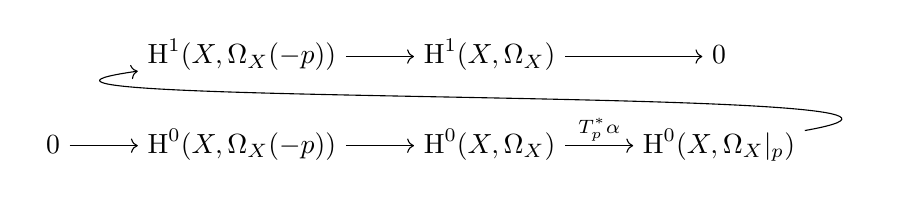
\begin{tikzpicture}[descr/.style={fill=white,inner sep=1.5pt}]
        \matrix (m) [
            matrix of math nodes,
            row sep=1.8em,
            column sep=2.5em,
            text height=1.5ex, text depth=0.25ex
        ]
        {  & \Hnm^1(X, \Omega_X(-p)) &  \Hnm^1(X, \Omega_X) & 0 &  \\
          0  & \Hnm^0(X, \Omega_X(-p)) & \Hnm^0(X, \Omega_X) & \Hnm^0(X, \Omega_X|_p) &  \\
        };

        \path[overlay,->, font=\scriptsize]
        
        (m-1-2) edge (m-1-3)
        (m-1-3) edge (m-1-4)
        (m-2-4) edge[out=10,in=188] (m-1-2)
        (m-2-1) edge (m-2-2)
        (m-2-2) edge (m-2-3)
        (m-2-3) edge node[above, yshift=-2pt] {$T_p^* \alpha$} (m-2-4)
        ;
\end{tikzpicture}
\end{center}
The proposition below follows from standard arguments in homological algebra:

\begin{proposition}\label{prop:dim_of_Albanese_image}
For a general point $p \in X$,
\begin{equation*}
\begin{aligned}
 \dim_{\mathbb{C}} \alpha(X) =\;& \rank T_p^* \alpha  \\ 
 =\;& n-h^0(X, \Omega_X(-p))  \\ 
 =\;& h^1(X, \Omega_X(-p))-h^1(X, \Omega_X).  \\ 
\end{aligned}
\end{equation*}
In particular,
\begin{equation*}
\begin{aligned}
  & \alpha \text{ is surjective} & \Longleftrightarrow\quad& h^0(X, \Omega_X(-p))=0 \\ 
  & \alpha \text{ is finite onto image} & \Longleftrightarrow\quad& h^0(X, \Omega_X(-p))=n-r \\ 
  & \alpha \text{ is constant} & \Longleftrightarrow\quad& h^0(X, \Omega_X(-p))=n \\ 
  & & \Longleftrightarrow\quad& h^1(X, \Omega_X(-p))=h^1(X, \Omega_X) \\ 
  & & \Longleftrightarrow\quad& n=0. \\ 
\end{aligned}
\end{equation*}
\end{proposition}
We will concentrate on the case where $\alpha$ is finite onto its image.\footnote{The general method remains valid in the broader setting, but the Gauss map then takes values in a different space.} Under this assumption, we set $Z = X$ and $A = \Alb(Z)$. The corresponding Gauss map is then a rational map:
% https://q.uiver.app/#q=WzAsNixbMCwwLCJcXHBoaV9aOiJdLFsyLDAsIlxcR3IocixUXjBBKSJdLFsxLDAsIloiXSxbMywwLCJcXEdyKG4tcixcXEhubV4wKFgsXFxPbWVnYV9YKSkiXSxbMywxLCJcXEhubV4wKFgsXFxPbWVnYV9YKC1wKSkiXSxbMSwxLCJwIl0sWzUsNCwiIiwwLHsic3R5bGUiOnsidGFpbCI6eyJuYW1lIjoibWFwcyB0byJ9fX1dLFsyLDEsIiIsMCx7InN0eWxlIjp7ImJvZHkiOnsibmFtZSI6ImRhc2hlZCJ9fX1dLFsxLDMsIlxcY29uZyIsMSx7InN0eWxlIjp7ImJvZHkiOnsibmFtZSI6Im5vbmUifSwiaGVhZCI6eyJuYW1lIjoibm9uZSJ9fX1dXQ==
\[\begin{tikzcd}[row sep={-1mm}]
	{\phi_Z:} &[-10mm] Z &[5mm] {\Gr(r,T^0A)} & [-7mm] {\Gr(n-r,\Hnm^0(X,\Omega_X))} \\
	& p && {\Hnm^0(X,\Omega_X(-p))}
	\arrow[dashed, from=1-2, to=1-3]
	\arrow["\cong"{description}, draw=none, from=1-3, to=1-4]
	\arrow[maps to, from=2-2, to=2-4]
\end{tikzcd}\]
and we have the isomorphisms 
\begin{equation*}
\begin{aligned}
   \mathbb{P}T^{*}_{0}A \cong\;& \mathbb{P}\Hnm^0(X,\Omega_X), \\ 
    \mathbb{P}\Lambda_{Z}=\;& \left\{\, (p,[\omega])  \in Z \times \mathbb{P}T^{*}_{0}A \;\middle|\; \omega(p)=0 \,\right\}  \\ 
    \cong\;& \left\{\,\rule{0mm}{3.2mm} (p,[\omega])  \in Z \times \mathbb{P}T^{*}_{0}A \;\middle|\; \omega \in \Hnm^0(X,\Omega_X(-p)) \,\right\}  \\ 
    \cong\;& \left(\phi_Z, \Id \right)^{-1} I_{n-r, 1},  \\ 
\end{aligned}
\end{equation*}
where 
$$I_{n-r, 1}:= \left\{\, \rule{0mm}{3.2mm} (V,[\omega])  \in \Gr(n-r,n) \times \Gr(1, n) \;\middle|\; \omega \in V \,\right\}$$ 
is the incidence variety relating $\Gr(n-r,n)$ and $\Gr(1, n)$. In that case, 
\begin{equation*}
\begin{aligned}
    \gamma_Z^{-1}([\omega])=\;& \left\{\, p  \in X  \;\middle|\; \omega(p)=0 \,\right\}  \\  
\end{aligned}
\end{equation*}
is the zero set of section $\omega \in \Hnm^0(X,\Omega_X)$. The number $(-1)^r \deg \gamma_Z$ is the index in the Poincaré--Hopf index formula, and the monodromy group $\Gal(\gamma_Z)$ serves as a more refined invariant, encoding subtler aspects of the geometry.

The next proposition shows when the Gauss map $\phi_Z$ is not generic injective.
\begin{proposition}
When $\alpha$ is finite onto its image,
\begin{equation*}
\begin{aligned}
  \;&  \phi_Z \text{ is not generic injective} \\ 
  \Longleftrightarrow\;\;& \text{For general $p \in X$, exists $q \neq p$ such that $h^0(X,\Omega_X(-p-q))=n-r$} \\ 
  \stackrel{\textcolor{purple}{\textbf{?}\footnotemark}}{\Longleftrightarrow}\;\;& \text{For general $p \in X$, exists $S \in X^{[2]}$ such that $p\in S$ and $h^0(X,\Omega_X \otimes \mathcal{I}_S)=n-r$} \\ 
  \Longleftrightarrow\;\;& \text{For all $p \in X$, exists $S \in X^{[2]}$ such that $p\in S$ and $h^0(X,\Omega_X \otimes \mathcal{I}_S)\geqslant n-r$.} \\ 
\end{aligned}
\end{equation*}
\end{proposition}
\footnotetext{When $n = r$, the map $\varphi_Z$ has a point as its target, so the equivalence is trivial.
When $n > r$, the implication ``$\Rightarrow$" is immediate. For the converse ``$\Leftarrow$", it suffices to show that the image of 
$$\left\{ S \in X^{[2]} \;\middle|\; h^0(X,\Omega_X \otimes \mathcal{I}_S)=n-r   \right\}$$
 under the map $\pi_X:X^{[2]} \longrightarrow X^{(2)} $ does not include the diagonal. Indeed, we can choose a section $s \in \Hnm^0(X,\Omega_X)$ that cuts out finitely many reduced points $p_1,\ldots,p_d$ in $X$. (Well this maybe not so true, since $\phi_Z$ is not always regular, such a section $s$ may vanish along some indeterminacy locus. However, for a general $s$, there will always be at least one isolated zero $p_1$, which is sufficient for our purposes.)
Then for any $S \in \pi_X^{-1}(p_1)$, we have 
$$\Hnm^0(X,\Omega_X \otimes \mathcal{I}_S)  \subsetneqq \Hnm^0(X,\Omega_X(-p_1)).$$
}
This last step relies on the following lemma, combined with the closedness of the tautological correspondence in $X \times X^{[2]}$.
\begin{lemma}
Let $m \in \mathbb{Z}_{>0}$. The function $$h^{\Omega}: X^{[m]} \longrightarrow \mathbb{Z}_{\geqslant 0} \qquad
 S \longmapsto h^0(X,\Omega_X \otimes \mathcal{I}_S)$$ 
is Zariski upper semicontinuous.
\end{lemma}
\begin{proofsketch}
Consider the coherent sheaf $\mathcal{F} \in \Coh(X^{[m]} \times X)$ characterized by the property
$$\mathcal{F}|_{\{S\} \times X} \cong \Omega_X \otimes \mathcal{I}_S,$$
The proposition then follows directly from the semicontinuity theorem \cite[28.1.1]{vakil2017rising}.
\end{proofsketch}

The stratification of $X^{[m]}$ by $h^{\Omega}$ offers a natural generalization of Brill--Noether theory beyond the setting of curves.

$\,$

At the end of this subsection, let us turn to the setting of a general abelian variety $A$ and a smooth subvariety $\iota_Z: Z \hookrightarrow A$, where $n = \dim_{\mathbb{C}} A$ and $r = \dim_{\mathbb{C}} Z$. Observe that $\iota_Z$ factors through the Albanese variety of $Z$:
% https://q.uiver.app/#q=WzAsMyxbMCwwLCJcXGlvdGFfWjogWiAgIl0sWzEsMCwiXFxBbGIoWikiXSxbMiwwLCJBIl0sWzAsMSwiXFxhbHBoYV9aIl0sWzEsMiwiXFxwaSJdXQ==
\[\begin{tikzcd}[column sep=large]
	{\iota_Z: Z  } & {\Alb(Z)} & A
	\arrow["{\alpha_Z}", from=1-1, to=1-2]
	\arrow["\pi", from=1-2, to=1-3]
\end{tikzcd}\]

We shall also assume that $Z$ generates $A$; it then follows that the map $\pi$ is surjective. The cotangent map of $\iota_Z$ at a point $p \in Z$ factors through $\Hnm^0(Z, \Omega_Z)$:
% https://q.uiver.app/#q=WzAsMyxbMCwwLCJUX3BeKiBcXGlvdGFfWjogVF9wXipBICAiXSxbMSwwLCJcXEhubV4wKFosIFxcT21lZ2FfWikiXSxbMiwwLCJUX3BeKloiXSxbMCwxLCIiLDAseyJzdHlsZSI6eyJ0YWlsIjp7Im5hbWUiOiJob29rIiwic2lkZSI6InRvcCJ9fX1dLFsxLDJdXQ==
\[\begin{tikzcd}[column sep=large]
	{T_p^* \iota_Z: T_p^*A  } & {\Hnm^0(Z, \Omega_Z)} & {T_p^*Z}
	\arrow[hook, from=1-1, to=1-2]
	\arrow[from=1-2, to=1-3]
\end{tikzcd}\]
For convenience, abbreviate $V := T_0^*A \cong T_p^*A$, and view $V$ as a subspace of $\Hnm^0(Z, \Omega_Z)$.
\begin{proposition}
Assume that $Z$ is embedded in $A$ and generates $A$, and let $V := T_0^*A$. Then
$$\dim_{\mathbb{C}} \Hnm^0(Z,\Omega_Z(-p)) \cap V =n-r \qquad \text{ for all $p \in Z$}$$
It follows that the Gauss map is a regular morphism
\[\begin{tikzcd}[row sep={-1mm}]
	{\phi_Z:} &[-10mm] Z &[5mm] {\Gr(r,T^0A)} & [-7mm] {\Gr(n-r,V)} \\
	& p && {\Hnm^0(Z,\Omega_Z(-p)) \cap V}
	\arrow[from=1-2, to=1-3]
	\arrow["\cong"{description}, draw=none, from=1-3, to=1-4]
	\arrow[maps to, from=2-2, to=2-4]
\end{tikzcd}\]
 Furthermore, 
\begin{equation*}
\begin{aligned}
  \;&  \phi_Z \text{ is not generic injective} \\ 
  \Longleftrightarrow\;\;& \text{For general $p \in Z$, exists $q \neq p$ such that $h^0(Z,\Omega_Z(-p-q)) \cap V =n-r$} \\ 
  \Longleftrightarrow\;\;& \text{For all $p \in Z$, exists $S \in Z^{[2]}$ such that $p\in S$ and $h^0(Z,\Omega_Z \otimes \mathcal{I}_S) \cap V=n-r$.} \\ 
\end{aligned}
\end{equation*}
\end{proposition}

\begin{ques}
For an $r$-dimensional smooth variety $Z$ whose Albanese map $\alpha_Z$ is an embedding, which subspaces $V \subset \Hnm^0(Z, \Omega_Z)$ can arise as the cotangent space of some abelian quotient variety of $\Alb(Z)$?
\end{ques}

The precise formulation of this question is somewhat ambiguous, and depending on the interpretation, it may turn out to be either relatively straightforward or extremely difficult. On the one hand, the classification of abelian subvarieties of $A$ via symmetric idempotents in $\End_{\mathbb{Q}}(A)$ is well established \cite[Theorem 5.3.2]{BL04}. On the other hand, explicitly computing $\End_{\mathbb{Q}}(A)$ can be highly nontrivial when $A$ is a non-simple Albanese variety—even in the case where $A$ arises from a curve.





\section{Families of subvarieties}

In this section, we move from the study of monodromy groups to a more direct analysis of the subvarieties themselves. Given an initial subvariety, one can naturally generate a family of subvarieties. Our goal here is to define these families and investigate their properties.

\begin{proposition}
All irreducible conic Lagrangian cycles in $T^*A$ are of the form $\Lambda_Z$ for some irreducible subvariety $Z \subset A$. This yields a one-to-one correspondence between irreducible conic Lagrangian cycles in $T^*A$ and irreducible subvarieties of $A$:
$$\left\{\text{ irreducible conic Lagrangian cycles in $T^*A$ }   \right\} \longleftrightarrow \left\{\text{ irreducible subvarieties in $A$ }   \right\}$$
\end{proposition}

\begin{proofsketch}
For any irreducible conic Lagrangian cycle $\mathbf{\Lambda} \subset T^*A$, let $Z$ denote the image of $\mathbf{\Lambda}$ under the natural projection $T^*A \to A$. Our goal is to show that $\mathbf{\Lambda} = \Lambda_Z$.
\begin{itemize}
\item By definition, $\mathbf{\Lambda} \subset T^*A|_Z$.
\item Since $\mathbf{\Lambda}$ is conic, we have $s(Z) \subset \mathbf{\Lambda}$, where $s : A \to T^*A$ denotes the zero section.
\item Since $\mathbf{\Lambda}$ is Lagrangian and $s(Z) \subset \mathbf{\Lambda}$, we have $\mathbf{\Lambda} \subset \Lambda_Z$.
\item Since $\Lambda_Z$ is irreducible with $\dim_{\mathbb{C}} \mathbf{\Lambda} = \dim_{\mathbb{C}} \Lambda_Z = n$, we have $\mathbf{\Lambda} = \Lambda_Z$.
\end{itemize}
\end{proofsketch}

Why do we shift attention from $Z$ to $\Lambda_Z$ as the main object of study? One reason is the uniformity of $\Lambda_Z$: it always has dimension $n$, and in most cases, the natural map $\Lambda_Z \to T_0^* A$ is generically finite, with fibers lying inside $A$.

\begin{definition}[Clean cycle]
An irreducible Lagrangian cycle $\mathbf{\Lambda} \subset T^*A$ is called clean if the composed projection
$$\mathbf{\Lambda} \longrightarrow T^*A \twoheadrightarrow T_0^*A$$
is generically finite.
\end{definition}

Another important reason is that the space of weighted clean conic Lagrangian cycles naturally acquires a convolution structure, arising from the group law on $A$, which plays a central role in the analysis.

\begin{proposition}
The group of weighted clean conic Lagrangian cycles
\begin{equation*}
\begin{aligned}
  \mathcal{L}(A):=\;& \left\{ \text{weighted clean conic Lagrangian cycles in }T^*A \right\}  \\ 
  =\;& \left\{ \raisebox{1.5mm}{$\displaystyle\sum_{\substack{Z_i \subset A \\ \text{irr clean}}}$}n_i \Lambda_{Z_i}\; \middle|\; n_i \in \mathbb{Z} \right\}  \\ 
\end{aligned}
\end{equation*}
has a natural convolution structure as follows: 
\begin{equation*}
\begin{aligned}
  \Lambda_{Z_1} \circ \Lambda_{Z_2}=\;& \text{ the clean part of }(a,\Id_{T_0^* A})_* \left( \Lambda_{Z_1} \times_{T_0^* A} \Lambda_{Z_2} \right) \\ 
  =\;& \overline{(a,\Id_{U})_* \left( \Lambda_{Z_1}|_U \times_{U} \Lambda_{Z_2}|_U \right)} \\ 
\end{aligned}
\end{equation*}
where 
$$U:=\left\{ \xi \in T_0^*A \; \middle|\; \rule{0mm}{3.4mm}\deg \phi_{Z_i}= \# \phi_{Z_i}^{-1}(\xi) \text{ for } i=1,2 \right\}$$
and $a: A \times A \longrightarrow A$ is the addition map in $A$. The general convolution is defined by $\mathbb{Z}$-linear extension.
\end{proposition}

\begin{proofsketch}
To establish the claim, it suffices to show that $\Lambda_{Z_1} \circ \Lambda_{Z_2}$ defines a weighted conic Lagrangian cycle. The conic property follows directly from the definition, while the Lagrangian condition can be verified at a general point $(p_1 + p_2, \xi) \in \Lambda_{Z_1} \circ \Lambda_{Z_2}$.
\end{proofsketch}

We now consider the projective versions of all objects involved, so that we may make use of properness. To simplify notation, we abbreviate $\mathbb{P}T^{*}_{0}A$ by $\mathbb{P}^{\vee}$.

\begin{lemma}\label{lem:mon_of_prod}\
\begingroup
\upshape
%\setlist{itemsep=-0.4em}
\renewcommand\labelenumi{(\theenumi)}
\begin{enumerate}[(1)]
\item Suppose that $\mathbb{P}\Lambda_{Z_1}, \mathbb{P}\Lambda_{Z_1} \subset \mathbb{P}T^*A$ admit monodromy representations $$\rho_{\gamma_{Z_i}}: \pi_1(U,\xi_0) \longrightarrow \Aut\left(\gamma_{Z_i}^{-1}(\xi_0)\right),$$ 
then $\mathbb{P}\Lambda_{Z_1} \times_{\mathbb{P}^{\vee}} \mathbb{P}\Lambda_{Z_2} \subset A\times A \times \mathbb{P}^{\vee}$ admits monodromy representation given by
$$(\rho_{\gamma_{Z_1}},\rho_{\gamma_{Z_2}}): \pi_1(U,\xi_0) \longrightarrow \Aut\left(\gamma_{Z_1}^{-1}(\xi_0) \times \gamma_{Z_2}^{-1}(\xi_0)\right),$$ 
\item When $Z_1=Z_2=Z$, we obtain an one-to-one correspondence:
$$\left\{ 
\begin{aligned}
  &\text{ irr components of } \mathbb{P}\Lambda_{Z} \times_{\mathbb{P}^{\vee}} \mathbb{P}\Lambda_{Z}  \\ 
  &\hspace{10mm}\text{ with a surjection to } \mathbb{P}^{\vee}
\end{aligned}
 \right\} \longleftrightarrow 
\left\{ 
\begin{aligned}
  &\Gal(\gamma_{Z})\text{-orbits of }  \\ 
  &\;\;\gamma_{Z}^{-1}(\xi_0) \times \gamma_{Z}^{-1}(\xi_0)
\end{aligned}
 \right\} 
 $$
\end{enumerate}
\endgroup
\end{lemma}
\begin{proofsketch}
Statement (1) holds by definition. The proof of (2) reduces to the following purely topological statement:
\begin{claim}
Let $\pi: E \longrightarrow B$ be a (unramified) covering space over a manifold $B$ with deck transformation group $G$, then
$$\left\{ \rule{0mm}{3.1mm}\text{ connected components of }E \times_B E \;\right\} \longleftrightarrow \left\{   \;G\text{-orbits of } \pi^{-1}(b_0) \times \pi^{-1}(b_0)\; \right\}. $$
\end{claim}
\noindent The claim follows directly from the correspondence between covering spaces over $B$ and $\pi_1(B)$-sets; see \cite[Theorem 1.38]{Ha02}.
\end{proofsketch}

Generalizing the argument of Lemma \ref{lem:mon_of_prod}, we arrive at the following lemma.

\begin{lemma}
For $d=\deg \gamma_{Z}$, $\xi_0 \in T_0^* A$ a general point, write
\begin{equation*}
\begin{aligned}
  \mathbb{P}\Lambda_{Z}^{\times d} :=\;&\;\; \mathbb{P}\Lambda_{Z} \times_{\mathbb{P}^{\vee}}\mathbb{P}\Lambda_{Z} \times_{\mathbb{P}^{\vee}} \cdots \times_{\mathbb{P}^{\vee}} \mathbb{P}\Lambda_{Z} && \subset A^d \times \mathbb{P}^{\vee}\\ 
  \gamma_{Z}^{-1}(\xi_0)^{d} :=\;& \gamma_{Z}^{-1}(\xi_0) \times \gamma_{Z}^{-1}(\xi_0) \times \cdots \times \gamma_{Z}^{-1}(\xi_0) && \subset A^d \\ 
\end{aligned}
\end{equation*}
\begingroup
\upshape
%\setlist{itemsep=-0.4em}
\renewcommand\labelenumi{(\theenumi)}
\begin{enumerate}[(1)]
\item we obtain an one-to-one correspondence:
$$\left\{ 
\begin{aligned}
  &\text{ irr components of } \mathbb{P}\Lambda_{Z}^{\times d}  \\ 
  &\hspace{0mm}\text{ with a surjection to } \mathbb{P}^{\vee}
\end{aligned}
 \right\} \longleftrightarrow 
\left\{ 
\begin{aligned}
  &\Gal(\gamma_{Z})\text{-orbits of }  \\ 
  &\hspace{8mm}\gamma_{Z}^{-1}(\xi_0) ^d
\end{aligned}
 \right\} 
 $$
\item Write
\begin{equation*}
\begin{aligned}
  \Delta_d :=\;&\left\{ (p_1,\ldots,p_d) \in A^d \;\middle|\; p_i=p_j \text{ for some } i \neq j  \right\} && \subset A^d \\ 
  \mathbb{P}\Lambda_{Z}^{[d]} :=\;& \overline{\left( \mathbb{P}\Lambda_{Z}^{\times d} \smallsetminus \left( \Delta_d \times \mathbb{P}^{\vee} \right) \right)|_U} && \subset A^d \times \mathbb{P}^{\vee}\\ 
\end{aligned}
\end{equation*}
Fix a general point $\xi_0 \in \mathbb{P}^{\vee}$ and a well-order for $\gamma_{Z}^{-1}(\xi_0)$, one can identify $S_d \cong \gamma_{Z}^{-1}(\xi_0)^d \smallsetminus \Delta_d$, and 
$$\left\{ 
\text{ irr components of } \mathbb{P}\Lambda_{Z}^{[d]}  
 \;\right\} \longleftrightarrow 
\left\{ \;\rule{0mm}{3.3mm}
\Gal(\gamma_{Z})\text{-orbits of }  S_d
 \;\right\} 
 $$
 In reference, $\Delta_d$ is usually called the big diagonal.
\end{enumerate}
\endgroup
\end{lemma}

From this point on, we fix an irreducible component of $\mathbb{P}\Lambda_{Z}^{[d]}$, denoted by $\mathbb{P}\Lambda_{Z}^{\univ}$. As we will see in Definition A, this variety generates all subvarieties within the families under consideration.

\begin{definition}[The subvariety $Z^{(m)}$]
For any tuple $(m) = (m_1, \ldots, m_d) \in \mathbb{Z}^d$, we define the weighted sum map
$$a^{(m)}: A^d \longrightarrow A \qquad (p_1,\ldots,p_d) \longmapsto \sum_{i=1}^{d} m_ip_i.$$
We also define 
$$\mathbb{P}\Lambda_{Z}^{(m)}: = \left( a^{(m)},\Id_{\mathbb{P}^{\vee}}  \right)_* \mathbb{P}\Lambda_{Z}^{\univ}.$$
as the (projectivized) weighted Lagrangian cycle in $\mathbb{P}T^*A$. The projective cycle $\mathbb{P}\Lambda_{Z}^{(m)}$ is irreducible but may appear with multiplicities. We can therefore write
$$\mathbb{P}\Lambda_{Z}^{(m)} = c_Z^{(m)}  \mathbb{P}\Lambda_{Z^{(m)}}$$
where $c_Z^{(m)} \in \mathbb{Z}_{>0}$ and $Z^{(m)} \subset A$ are uniquely determined. This gives rise to a family of subvarieties parametrized by $\mathbb{Z}^d$.
\end{definition}

The next lemma gathers some basic properties of $Z^{(m)}$. Observe that $S_d=\Aut\left(\gamma_{Z}^{-1}(\xi_0)\right)$ acts naturally on $\mathbb{Z}^d$ via
$$g(m)=\left(m_{g(1)},\ldots , m_{g(d)}\right) \in \mathbb{Z}^d.$$

\begin{lemma}\
\begingroup
\upshape
%\setlist{itemsep=-0.4em}
\renewcommand\labelenumi{(\theenumi)}
\begin{enumerate}[(1)]
\item For all $g\in \Gal(\gamma_{Z})$, we have $ Z^{g(m)}=Z^{(m)}$, $c_Z^{g(m)}=c_Z^{(m)}$;
\item For $(m)=(1,0,\ldots,0)\in \mathbb{Z}^d$, $Z^{(m)}=Z$;
\item For all $(m), (m') \in \mathbb{Z}^d$, we have  $\mathbb{P}\Lambda_{Z}^{(m)} \circ \mathbb{P}\Lambda_{Z}^{(m')} \supseteq \mathbb{P}\Lambda_{Z}^{(m+m')}$;
\item The group $\left< \mathbb{P}\Lambda_{Z^{(m)}} \right>_{\Abel}$ is closed under the convolution product.
\end{enumerate}
\endgroup
\end{lemma}



\section{Monodromy group}\label{sec:mon_examples}

\subsection{Curves in Prym variety with small monodromy group}
This subsection is devoted to presenting an example that demonstrates Proposition \ref{prop: smallmongp}.


\begin{setting}\label{set: Prym}
Suppose $C'$ is a smooth projective curve of genus $g(C')$, and let $B$ be an effective (possibly zero) divisor on $C'$. For any line bundle $\eta \in \Pic(C')$ such that $\eta^{\otimes 2} \cong \mathcal{O}_{C'}(B)$, one obtains a double cover $h: C \to C'$ of smooth projective curves, ramified precisely over $B$. The associated involution on $C$ is denoted by $\iota$, and the triple $(C, C', h)$ is referred to as the Prym pair.

Recall that the Prym variety $A := \Prym(C/C')$ is defined as the connected component of the identity in 
$$\ker \left[\Nm:\rule{0mm}{3.4mm}\Jac(C) \longrightarrow \Jac(C') \right].$$ 
The Abel--Prym map is defined by
$$\AP_{C/C'}: C \longrightarrow A \qquad p \longmapsto \mathcal{O}_{C}(p-\iota(p)).$$
\end{setting}

The classical theory treats the case where the Prym variety $A$ is principally polarized—this occurs exactly when $B = \varnothing$ or $B =\{p_0, q_0\}$, that is, when $h$ is either unramified or ramified at two points.\footnote{See \cite[Theorem 3.2.6]{CK22} for the proof.} For clarity and focus, we restrict our attention to these cases. Table \ref{table:Prym_numerical_data} lists the relevant numerical data.\footnote{As usual, $n=\dim_{\mathbb{C}} A$ is the dimension of the abelian variety.}

{
\def\arraystretch{1.2}
\begin{table}[ht]
\begin{tabular}{c|c|c|c}
\hline
                  & $g(C)$ & $g(C')$ & $\deg \eta$ \\ \hline
$B = \varnothing$ & $2n+1$ & $n+1$   & $0$         \\ \hline
$B =\{p_0, q_0\}$ & $2n$   & $n$     & $1$         \\ \hline
\end{tabular}
\medskip
\caption{numerical data of Prym pair}
\label{table:Prym_numerical_data}
\vspace*{-\baselineskip}
\end{table}
}
The Abel–Prym map $\AP_{C/C'}$ does not always behave as nicely as the Abel–Jacobi map; it may fail to be an embedding. When $C$ is hyperelliptic, the map $\AP_{C/C'}$ fails to be generically injective, and therefore falls outside the scope of our discussion. When $C$ is non-hyperelliptic, we may regard it as a subvariety of $A$ for our purposes, although it may be not strictly embedded.\footnote{For a detailed description of the map $\AP_{C/C'}$, see \cite[Proposition 12.5.2, Corollary 12.5.6]{BL04}. Although $\AP_{C/C'}$ may collapse $p_0$ and $q_0$, this does not affect the relevant computation of $\Gal(\gamma_Z)$.} However, it remains unclear whether $C$ is stable under any translation in $A$.

In the Prym setting, the corresponding Gauss map $\gamma_C$ factors through $h$: 
% https://q.uiver.app/#q=WzAsMTEsWzAsMCwiXFxnYW1tYV9DOiJdLFsxLDAsIkMiXSxbMiwwLCJDJyJdLFszLDAsIlxcbWF0aGJie1B9XntuLTF9Il0sWzUsMCwiXFxtYXRoYmJ7UH1cXCFcXGxlZnQoIEheMChcXG9tZWdhX3tDJ30gXFxvdGltZXMgXFxldGEpXiogXFxyaWdodCkiXSxbNSwxLCJcXEdyXFxsZWZ0KG4tMSwgSF4wKFxcb21lZ2Ffe0MnfSBcXG90aW1lcyBcXGV0YSlcXHJpZ2h0KSJdLFs1LDIsIkheMFxcbGVmdChcXG9tZWdhX3tDJ30gXFxvdGltZXMgXFxldGEoLXApXFxyaWdodCkiXSxbMiwyLCJwIl0sWzEsMiwiXFx0aWxkZXtwfSJdLFs0LDAsIj0iXSxbNCwxLCJcXGNvbmciXSxbOCw3LCIiLDAseyJzdHlsZSI6eyJ0YWlsIjp7Im5hbWUiOiJtYXBzIHRvIn19fV0sWzIsMywifFxcb21lZ2Ffe0MnfSBcXG90aW1lcyBcXGV0YXwiXSxbMSwyLCJoIl0sWzcsNiwiIiwwLHsic3R5bGUiOnsidGFpbCI6eyJuYW1lIjoibWFwcyB0byJ9fX1dXQ==
\[\begin{tikzcd}[column sep=10mm,row sep=-2mm]
	{\gamma_C:} &[-12mm] C & {C'} & [5mm] {\mathbb{P}^{n-1}} & [-12mm]{=} &[-12mm] {\hspace{-10mm}\mathbb{P}\!\left( \Hnm^0(\omega_{C'} \otimes \eta)^* \right)} \\
	&&&& \cong & {\Gr\left(n-1, \Hnm^0(\omega_{C'} \otimes \eta)\right)} \\[1mm]
	& {\tilde{p}} & p &&& {\Hnm^0\left(\omega_{C'} \otimes \eta(-p)\right)}
	\arrow["h", from=1-2, to=1-3]
	\arrow["{|\omega_{C'} \otimes \eta|}", from=1-3, to=1-4]
	\arrow[maps to, from=3-2, to=3-3]
	\arrow[maps to, from=3-3, to=3-6]
\end{tikzcd}\]


\begin{eg} \label{eg:bielliptic}
Let $C'$ be a non-hyperelliptic bielliptic curve, and let $\pr: C' \to E$ denote a $2:1$ covering onto an elliptic curve. For any nontrivial $2$-torsion line bundle $\eta_0 \in \Pic^0(E)[2]$, the pullback $\eta := \pr^* \eta_0$ satisfies $\eta^{\otimes 2} \cong \mathcal{O}_{C'}$ and the map $|\omega_{C'} \otimes \eta|$ factors through $\pr$.
\end{eg}
\begin{proof}[{Proof of Example \ref{eg:bielliptic}}]
For any $x \in C'$, write $x_0:= \pr(x)$, then
$$ \deg \eta_0^{\vee} (x_0)=1 \quad \Longrightarrow \quad \text{ there exists } y_0 \in E \text{ such that } \eta_0^{\vee} (x_0)=\mathcal{O}_E(y_0).$$
Write $\pr^{-1}(x_0)=\{x,x'\}$, $\pr^{-1}(y_0)=\{y,y'\}$, we get
\begin{equation*}
\begin{aligned}
\;& \eta_0^{\vee} (x_0)=\mathcal{O}_E(y_0) && \\ 
\Longrightarrow\;& \eta^{\vee}(x+x')= \mathcal{O}_{C'}(y+y') && \text{Via pulling back along $\pr$} \\ 
  \Longrightarrow\;& h^0 \left(\rule{0mm}{3mm} \eta^{\vee}(x+x')\right) = 1 && \\ 
  \Longleftrightarrow\;& h^0 \left(\rule{0mm}{3mm}\omega_{C'} \otimes \eta(-x-x')\right) = n - 1 && \text{Via Riemann--Roch}\\
  \Longleftrightarrow\;& \Hnm^0 \left(\rule{0mm}{3mm}\omega_{C'} \otimes \eta(-x)\right) \cong  \Hnm^0 \left(\rule{0mm}{3mm}\omega_{C'} \otimes \eta(-x')\right) \qquad && \\ 
  \Longleftrightarrow\;& |\omega_{C'} \otimes \eta|(x)=|\omega_{C'} \otimes \eta|(x') &&
\end{aligned}
\end{equation*}
\end{proof}

The next proposition tells us, for the most time the resulting curve $C \subset A$ is not invariant under any non-trivial translation of $A$. 

\begin{proposition}\label{prop:Galois_condition}
In Example \ref{eg:bielliptic}, let $C$ be the curve corresponding to $\eta \in \Pic^{0}(C')[2]$. If $\Gal(C/E) \cong \mathbb{Z}/2\mathbb{Z} \oplus \mathbb{Z}/2\mathbb{Z}$, then $C$ admits three intermediate quotients over $E$. Denote them by $C'$, $C_1$, and $C_2$, where $C_1$ and $C_2$ are the two intermediate curves different from $C'$.

% https://q.uiver.app/#q=WzAsMTIsWzAsMCwiQyJdLFswLDEsIkMnIl0sWzIsMCwiQyJdLFsyLDEsIkMnIl0sWzIsMiwiRSJdLFsyLDMsIlxcbWF0aGJie1B9XjEiXSxbMCwyLCJFIl0sWzAsMywiXFxtYXRoYmJ7UH1eMSJdLFsxLDEsIkNfMSJdLFszLDEsIkNfMiJdLFsyLDQsIlxcR2FsKEMvRSkgXFxjb25nIFxcbWF0aGJie1p9LzJcXG1hdGhiYntafSBcXG9wbHVzIFxcbWF0aGJie1p9LzJcXG1hdGhiYntafSJdLFswLDQsIlxcR2FsKEMvRSkgXFxjb25nIFxcbWF0aGJie1p9LzRcXG1hdGhiYntafSJdLFsxLDZdLFswLDEsImgiXSxbNiw3XSxbMiwzLCJoIl0sWzMsNF0sWzQsNV0sWzgsNF0sWzksNF0sWzIsOSwiaF8yIl0sWzIsOCwiaF8xIiwyXV0=
\[\begin{tikzcd}[ampersand replacement=\&,column sep={10mm,between origins},row sep=5mm]
	C \&[30mm]\&[2mm] C \\
	{C'} \& {C_1} \& {C'} \& {C_2} \\
	E \&\& E \\
	{\mathbb{P}^1} \&\& {\mathbb{P}^1} \\[-3mm]
	{\Gal(C/E) \cong \mathbb{Z}/4\mathbb{Z}} \&\& {\Gal(C/E) \cong \mathbb{Z}/2\mathbb{Z} \oplus \mathbb{Z}/2\mathbb{Z}}
	\arrow["h", from=1-1, to=2-1]
	\arrow["{h_1}"', from=1-3, to=2-2]
	\arrow["h", from=1-3, to=2-3]
	\arrow["{h_2}", from=1-3, to=2-4]
	\arrow[from=2-1, to=3-1]
	\arrow[from=2-2, to=3-3]
	\arrow[from=2-3, to=3-3]
	\arrow[from=2-4, to=3-3]
	\arrow[from=3-1, to=4-1]
	\arrow[from=3-3, to=4-3]
\end{tikzcd}\]
If either $\Gal(C/E) \cong \mathbb{Z}/4\mathbb{Z}$, or $\Gal(C/E) \cong \mathbb{Z}/2\mathbb{Z} \oplus \mathbb{Z}/2\mathbb{Z}$ with the coverings $h_i:C \to C_i$ ramified, then the curve $C \subset A$ is not fixed under any non-trivial translation on $A$.
\end{proposition}

\begin{proof}
We prove by contradiction.
Assume there exists a non-trivial translation $\sigma:A\to A$ preserving $C$. Then the restriction $\sigma|_{C}:C \to C$ is an automorphism, and the induced map
$$h_{\sigma}: C \longrightarrow C/\sigma$$
is an unramified double covering. Since $\sigma$ is a translation, the Gauss map $\gamma_C$ necessarily factors through $h_{\sigma}$:
% https://q.uiver.app/#q=WzAsNixbMCwwLCJcXGdhbW1hX0PvvJoiXSxbMSwwLCJDIl0sWzIsMCwiQyciXSxbMywwLCJFIl0sWzQsMCwiXFxtYXRoYmJ7UH1ee24tMX0iXSxbMiwxLCJDL1xcc2lnbWEiXSxbMSwyLCIyOjEiXSxbMiwzLCIyOjEiXSxbMyw0LCJcXHN1YnNldCIsMSx7InN0eWxlIjp7ImJvZHkiOnsibmFtZSI6Im5vbmUifSwiaGVhZCI6eyJuYW1lIjoibm9uZSJ9fX1dLFsxLDUsImhfe1xcc2lnbWF9IiwyXSxbNSwzLCJcXGV4aXN0cyEiLDIseyJzdHlsZSI6eyJib2R5Ijp7Im5hbWUiOiJkYXNoZWQifX19XV0=
\[\begin{tikzcd}[ampersand replacement=\&,column sep=15mm,row sep=5mm]
	{\gamma_C:} \&[-17mm] C \& {C'} \& E \&[-13mm] {\mathbb{P}^{n-1}} \\
	\&\& {C/\sigma}
	\arrow["{2:1}", from=1-2, to=1-3]
	\arrow["{h_{\sigma}}"', from=1-2, to=2-3]
	\arrow["{2:1}", from=1-3, to=1-4]
	\arrow["\subset"{description}, draw=none, from=1-4, to=1-5]
	\arrow["{\exists!}"', dashed, from=2-3, to=1-4]
\end{tikzcd}\]
Without loss of generality, we may assume that $\deg(h_\sigma)=2$. By assumption, $C/\sigma$ coincides with $C'$, and $\sigma|_C$ is the involution $\iota$ associated with the cover $h:C\to C'$, which extends to an involution $\tilde\iota$ of $A$. According to \cite[Proposition 12.4.2]{BL04}, $\tilde\iota$ is a reflection. Hence $\sigma \circ \tilde\iota^{-1}$ is another reflection fixing $C$, which is impossible.

\end{proof}

%Maybe I should check \cite{CMS21,JC92} for more information on Prym varieties of bielliptic curves.

\begin{proof}[Proof of Proposition \ref{prop: smallmongp}]
From Example \ref{eg:bielliptic}, we know that $\deg \gamma_C = 4$, hence by Lemma \ref{lem:wreath_product} we get
$$M_C = \Mon(\gamma_C) \subseteq S_4^{\oplus d/4} \rtimes S_{d/4}.$$

Assuming further that $\Gal(C/E) \cong \mathbb{Z}/4\mathbb{Z}$, Proposition \ref{prop:Galois_condition} implies that $C \subset A$ is divisible. In this case, by \cite[p.~5, Corollary (1)]{JKLM22}, the associated Tannaka group is big, namely
$$W_C\cong\; S_2^{\oplus d/2} \rtimes S_{d/2}.$$
\end{proof}


\subsection{Criteria for big monodromy group}

Proposition \ref{prop: smallmongp} shows that a small monodromy group can indeed occur, even in the case of curves. Nevertheless, there exist criteria ensuring that the monodromy group is large, which we describe in this subsection.



\begin{definition}[big monodromy group]\label{def:big_mono}
We refer to the big monodromy group as any group of the following types:
{
\def\arraystretch{1.2}
\begin{table}[ht]
\begin{tabular}{l|r|r}
\hline
\multicolumn{1}{c|}{notation}               & \multicolumn{1}{c|}{name}   & \multicolumn{1}{c}{alias}                     \\ \hline
$W(A_{m+1})=S_m$                            & full symmetric group        &                           \\ \hline
$\hspace{4mm}W(C_{m})=S_2^{\oplus m} \rtimes S_m$       & signed symmetric group      & hyperoctahedral group     \\ \hline
$\hspace{4mm}W(D_{m})=(S_2^{\oplus m})_{0} \rtimes S_m$ & even-signed symmetric group & demihyperoctahedral group \\ \hline
\end{tabular}
\medskip
\caption{big monodromy group}
\label{table:big_mono}
\vspace*{-\baselineskip}
\end{table}
}

In practice, the term ``big monodromy group'' refers to the full symmetric group $S_n$ when the subset $Z \subset A$ is not symmetric, and to the (even-)signed symmetric group when $Z \subset A$ is symmetric.

\end{definition}


\begin{proposition}[See {\cite[p111]{Ar85I}} for a detailed proof]\label{prop:mon_of_embedded_curve}
Suppose that $\iota_C: C \subseteq \mathbb{P}^{n-1}$ is an irreducible nondegenerate\footnote{A curve $C \subseteq \mathbb{P}^{n-1}$ is said to be nondegenerate if it is not contained in any hyperplane $H \subseteq \mathbb{P}^{n-1}$.} curve of degree $d$, then $\Mon(\iota_C) \cong S_d$.
\end{proposition}

\begin{proofsketch}
Because $S_d$ is generated by its transpositions, we are reduced to verifying that:
\begin{itemize}
\item $\Mon(\iota_C)$ acts doubly transitively on the fiber;
\item $\Mon(\iota_C)$ contains a transposition.
\end{itemize}
\end{proofsketch}






In fact, a degree $2:1$ map does not give rise to any exceptional monodromy groups beyond those listed in Table \ref{table:big_mono}.



\begin{proposition}\label{prop:mon_of_nonembedded_curve2}
Let $\iota_{C'} : C' \hookrightarrow \mathbb{P}^{n-1}$ be an irreducible nondegenerate curve of degree $d/2$, and let $\covermap: C \to C'$ be a degree $2$ ramified covering. Then $$\Mon(\iota_{C'} \circ \covermap) \cong W(C_{d/2}) \text{ or } W(D_{d/2}).$$
\end{proposition}

\begin{proofsketch}
By Lemma \ref{lem:wreath_product} we know that $\Mon(\iota_{C'} \circ \covermap) \subseteq W(C_{d/2})$.
By Lemma \ref{lem: type_C_Weyl_group2}, we are reduced to verifying that:
\begin{itemize}
\item The quotient map $\Mon(\iota_{C'} \circ \covermap) \longrightarrow \Mon(\iota_{C'}) \cong S_{d/2}$ is surjective;
\item (signed doubly transitive) $\Mon(\iota_{C'} \circ \covermap)$ acts transitively on pairs $(x,y)$ with $x\neq \pm y$. 
\end{itemize}
\end{proofsketch}

\begin{lemma}\label{lem: type_C_Weyl_group2}
Let $G$ be a subgroup of $W(C_{m})$, acting naturally on the set ${\pm 1, \ldots, \pm m}$. If the projection $G \to S_m$ is surjective  then 
$$G \cong  W(C_{m}) \text{ or } W(D_{m}) \text{ or } S_2 \times S_m \text{ or } S_{m}.$$
\end{lemma}

\begin{proofsketch}
Let $H$ denote the kernel of the natural quotient map $G \to S_m$. Then $H \subseteq (S_2)^{\oplus m}$ is stable under the action of $S_n$. There are only four possible forms that $H$ can take:\footnote{Here is a brief argument showing that $H$ must be one of $0$, $S_2$, $(S_2^{\oplus m})_0$, or $S_2^{\oplus m}$. If $H$ contains an element $h = (a_1, \ldots, a_m)$ with $a_i \neq a_j$ for some $i \neq j$, then $$(ij)h + h = (1,\ldots,\underset{\underset{i\text{-th}}{\uparrow}}{-1},\ldots,\underset{\underset{j\text{-th}}{\uparrow}}{-1},\ldots,1) \in H,$$ 
implying $(S_2^{\oplus m})_0 \subseteq H$. Hence, $H$ must be either $(S_2^{\oplus m})_0$ or $S_2^{\oplus m}$. Otherwise, if all $h \in H$ have identical coordinates, then $H$ is either $0$ or $S_2$.}
\begin{itemize}
\item $H=0$. Then $G\cong S_m$.
\item $H=\left< (-1,\ldots,-1) \right> \cong S_2$. Then $G\cong S_2 \times S_m$.
\item $H=(S_2^{\oplus m})_{0}$. Then $G$ is a index $2$ subgroup of $W(C_{m})$, so $G \cong W(D_{m})$.\footnote{Check \href{https://math.stackexchange.com/questions/3202823/wikipedia-inconsistency-with-the-index-2-subgroups-of-the-hyperoctahedral-group}{stackexchange discussions}} 
\item $H=S_2^{\oplus m}$. Then $G=W(C_{m})$.
\end{itemize}

\end{proofsketch}


\begin{proposition}\label{prop:mon_of_nonembedded_curve}
Let $\iota_{C'} : C' \hookrightarrow \mathbb{P}^{n-1}$ be an irreducible nondegenerate curve of degree $d/2$, and let $\covermap: C \to C'$ be a degree $2$ ramified covering, with ramification occurring at at least one smooth point of $C'$. Then $\Mon(\iota_{C'} \circ \covermap) \cong S_2^{\oplus d/2} \rtimes S_{d/2}$ is the hyperoctahedral group/signed symmetric group.
\end{proposition}

\begin{proofsketch}
By Lemma \ref{lem:wreath_product} we know that $\Mon(\iota_{C'} \circ \covermap) \subseteq S_2^{\oplus d/2} \rtimes S_{d/2}$.
By Lemma \ref{lem: type_C_Weyl_group}, we are reduced to verifying that:
\begin{itemize}
\item The quotient map $\Mon(\iota_{C'} \circ \covermap) \longrightarrow \Mon(\iota_{C'}) \cong S_{d/2}$ is surjective;
\item $\Mon(\iota_{C'} \circ \covermap)$ contains a transposition of a pair of points in the fiber of $\covermap$.
\end{itemize}
\end{proofsketch}

\begin{lemma}\label{lem: type_C_Weyl_group}
Let $G$ be a subgroup of $S_2^{\oplus m} \rtimes S_m$, acting naturally on the set ${\pm 1, \ldots, \pm m}$. If the projection $G \to S_m$ is surjective and the transposition $\sigma_0$ of $\pm 1$ lies in $G$, then $G = S_2^{\oplus m} \rtimes S_m$.
\end{lemma}

\begin{proofsketch}
Let $\varepsilon_i$ denote the transposition of $\pm i$. For any $\sigma \in S_m$, choose a lift $\tilde{\sigma} \in G$, then 
$$\varepsilon_{\sigma(1)}=\tilde{\sigma} \circ \sigma_0 \circ \tilde{\sigma}^{-1}   \in G.$$
Thus, $S_2^{\oplus m} \subset G$, and since $G$ maps onto $S_m$, we obtain $G = S_2^{\oplus m} \rtimes S_m$.
\end{proofsketch}


%When ramification occurring only in the smooth point of $C'$, I try to collect the following links:
%\href{https://mathoverflow.net/questions/310299/characterizing-subgroups-of-semidirect-products-with-a-fixed-intersection-with-t}{subgroups of semidirect products}
%\href{https://mathoverflow.net/questions/321698/first-group-cohomology-for-the-standard-representation-of-s-n-over-mathbbf}{first group cohomology for the standard representation of $S_n$}


\subsection{Curves with big monodromy group}

The availability of these criteria permits the systematic construction of numerous cases where the associated monodromy group is large.

\begin{eg}
Let $C$ be a smooth curve of genus $g$ embedded in its Jacobian $A := \Jac(C)$ via the Abel–Jacobi map $\AJ_C: C \hookrightarrow A$.

When $C$ is non-hyperelliptic, the corresponding Gauss map 
$$|\omega_C|: C\longrightarrow \mathbb{P}^{g-1}$$
makes $C$ as an irreducible nondegenerate curve of degree $2g-2$, by Proposition \ref{prop:mon_of_embedded_curve} we get
$$\Gal(\gamma_C) \cong S_{2g-2}.$$

When $C$ is hyperelliptic, the corresponding Gauss map is $2:1$ onto a rational normal curve $R \subset \mathbb{P}^{g-1}$:
% https://q.uiver.app/#q=WzAsMyxbMCwwLCJ8XFxvbWVnYV9DfDogQyJdLFsyLDAsIlxcbWF0aGJie1B9XntnLTF9Il0sWzEsMCwiUiJdLFswLDIsIjI6MSIsMCx7InN0eWxlIjp7ImhlYWQiOnsibmFtZSI6ImVwaSJ9fX1dLFsyLDEsIiIsMCx7InN0eWxlIjp7InRhaWwiOnsibmFtZSI6Imhvb2siLCJzaWRlIjoidG9wIn19fV1d
\[\begin{tikzcd}
	{|\omega_C|: C} & R & {\mathbb{P}^{g-1}}
	\arrow["{2:1}", two heads, from=1-1, to=1-2]
	\arrow[hook, from=1-2, to=1-3]
\end{tikzcd}\]
By Proposition \ref{prop:mon_of_nonembedded_curve} we get
$$\Gal(\gamma_C) \cong S_2^{\oplus g-1} \rtimes S_{g-1}.$$
\end{eg}



The Prym case is more intricate, since the associated monodromy group may fail to be large. To proceed, we fix Setting \ref{set: Prym} and impose the additional condition that $C$ be non-hyperelliptic, thereby excluding trivial counterexamples.

\begin{lemma}
When $\gon(C')>4$, $|\omega_{C'} \otimes \eta|$ is injective. As a result, the monodromy group is big.
\end{lemma}

\begin{proof}
Suppose that $|\omega_{C'} \otimes \eta|$ is not injective, we need to find a line bundle of degree $4$ and rank $\geqslant 1$. In fact, for $p\neq q$,
\begin{equation*}
\begin{aligned}
\;& |\omega_{C'} \otimes \eta|(p)=|\omega_{C'} \otimes \eta|(q) &&\\
  \Longleftrightarrow\;& h^0 \left(\omega_{C'} \otimes \eta\right) -  h^0 \left(\omega_{C'} \otimes \eta(-p-q)\right) = 1\qquad && \text{By \cite[19.2.8]{vakil2017rising}}\\ 
  \Longleftrightarrow\;& h^0 \left(\omega_{C'} \otimes \eta(-p-q)\right) = n - 1 && \text{Since $\dim_{\mathbb{C}} A = n$}\\
  \Longleftrightarrow\;& h^0 \left( \eta^{\vee}(p+q)\right) = 1 && \text{Via Riemann--Roch}\\   
\end{aligned}
\end{equation*}
When $B=\varnothing$, write $\eta^{\vee}(p+q)=\mathcal{O}_{C'}(p'+q')$, then
$$\mathcal{O}_{C'}(2p+2q) = \left(\eta^{\vee}\right)^{\otimes 2}(2p+2q) = \mathcal{O}_{C'}(2p'+2q') \hspace{25mm}\in g_4^1;$$
When $B=\{p_0,q_0\}$, write $\eta^{\vee}(p+q)=\mathcal{O}_{C'}(p')$, then
$$\mathcal{O}_{C'}(2p+2q) = \left(\eta^{\vee}\right)^{\otimes 2}(2p+2q+p_0+q_0) = \mathcal{O}_{C'}(2p'+p_0+q_0) \quad\in g_4^1.$$
\end{proof}

\begin{remark}
Based on the strategy used in the proof of Lemma 2.10, we can in fact obtain stronger results. For $p \in C'$,
\begin{equation*}
\begin{aligned}
\;& |\omega_{C'} \otimes \eta|\text{ is ramified at $p$} && \text{(i.e., the tangent map is $0$ at $p$)}\\
  \Longleftrightarrow\;& h^0 \left(\omega_{C'} \otimes \eta\right) -  h^0 \left(\omega_{C'} \otimes \eta(-2p)\right) = 1\qquad && \text{By \cite[19.2.9]{vakil2017rising}}\\ 
  \Longleftrightarrow\;& h^0 \left(\omega_{C'} \otimes \eta(-2p)\right) = n - 1 && \text{Since $\dim_{\mathbb{C}} A = n$}\\
  \Longleftrightarrow\;& h^0 \left( \eta^{\vee}(2p)\right) = 1 && \text{Via Riemann--Roch}\\   
\end{aligned}
\end{equation*}


For the remainder of this discussion, we focus exclusively on the case $B = \varnothing$. Combining both,
\begin{equation*}
\begin{aligned}
\;& |\omega_{C'} \otimes \eta|\text{ is not generically injective} \\
  \Longleftrightarrow\;&\text{For any } p \in C', \text{ there exist } q \in C' \text{ such that } h^0 \left( \eta^{\vee}(p+q)\right) = 1 \\   
\Longleftrightarrow\;&\text{For any } p \in C', \text{ there exist } q \in C' \text{ such that }  \eta^{\vee}+p \in C'+C'-q \\  
\Longleftrightarrow\;&  \eta^{\vee}+C' \subseteq C'+ C'- C'. \\ 
\end{aligned}
\end{equation*}
\end{remark}



Gonality is not the only invariant forcing the monodromy group to be large. Indeed, the Castelnuovo–Severi inequality implies that Example \ref{eg:bielliptic} is the sole instance of a non-trivial small monodromy group when $g(C') > 9$.

\begin{fact}[{Castelnuovo--Severi inequality, \cite[p26, Corollary]{Kani84}}]
Let $C$ be a smooth projective curve equipped with two ramified coverings $f_i: C \to C_i$ of degrees $d_i$ $(i=1,2)$. Suppose that there is no morphism $h: C \to \tilde{C}$ with $\deg(h) > 1$ such that both $f_1$ and $f_2$ factor through $h$. Then
$$g(C) \leqslant d_1 \cdot g(C_1) + d_2 \cdot g(C_2) + (d_1-1)(d_2-1).$$
\end{fact}

\begin{proposition}
If, in Setting \ref{set: Prym}, we additionally require that $C'$ be non-hyperelliptic and non-bielliptic, and $h: C \longrightarrow C'$ is étale, then any such curve with $g(C') \leqslant 9$ must have big monodromy group.
\end{proposition}

\begin{proof}
Assume that $C'$ and $\eta$ satisfies
$$\eta^{\vee}+C' \subseteq C'+ C'- C'.$$
$\;$\\
{\bfseries Step 1.} we can find two distinct $g_4^1$ of $C'$.

For any $p \in C'$, there exist $q,p',q' \in C'$ such that  
\[
\eta^{\vee}(p+q) = \mathcal{O}_{C'}(p'+q') .
\]
This implies  
\[
\mathcal{O}_{C'}(2p+2q) = \mathcal{O}_{C'}(2p'+2q') ,
\]
which defines a degree-$4$ covering $f_1\colon C' \to \mathbb{P}^1$ ramified at $p,q,p',q'$.  
Choosing $\tilde{p} \in C'$ outside the ramification locus of $f_1$ and repeating the construction yields another $g^1_4$, denoted $f_2\colon C' \to \mathbb{P}^1$.

$\;$\\
{\bfseries Step 2.} If $f_1$ and $f_2$ factor through a common map $h\colon C' \to \tilde{C}$ with $\deg(h) > 1$, then $C'$ is hyperelliptic or bielliptic.  

Indeed, in this case $\deg(h) = 2$, and the Castelnuovo--Severi inequality applied to $(\tilde{C}, \tilde{f}_1, \tilde{f}_2)$ gives $g(\tilde{C}) \leqslant 1$, so $\tilde{C}$ is either $\mathbb{P}^1$ or an elliptic curve.

% https://q.uiver.app/#q=WzAsNCxbMSwxLCJcXHRpbGRle0N9Il0sWzAsMiwiXFxtYXRoYmJ7UH1eMSJdLFsyLDIsIlxcbWF0aGJie1B9XjEiXSxbMSwwLCJDIl0sWzAsMSwiXFx0aWxkZXtmfV8xIl0sWzAsMiwiXFx0aWxkZXtmfV8yIiwyXSxbMywwLCJoIiwyXSxbMywxLCJmXzEiLDIseyJjdXJ2ZSI6Mn1dLFszLDIsImZfMiIsMCx7ImN1cnZlIjotMn1dXQ==
\[\begin{tikzcd}[ampersand replacement=\&,row sep=5mm]
	\& C \\
	\& {\tilde{C}} \\
	{\mathbb{P}^1} \&\& {\mathbb{P}^1}
	\arrow["h"', from=1-2, to=2-2]
	\arrow["{f_1}"', curve={height=12pt}, from=1-2, to=3-1]
	\arrow["{f_2}", curve={height=-12pt}, from=1-2, to=3-3]
	\arrow["{\tilde{f}_1}", from=2-2, to=3-1]
	\arrow["{\tilde{f}_2}"', from=2-2, to=3-3]
\end{tikzcd}\]

$\;$\\
{\bfseries Step 3.} If $C'$ is neither hyperelliptic nor bielliptic, then the Castelnuovo--Severi inequality yields $g(C') \leqslant 9$.
\end{proof}




 






\section{delete later}
\begin{ques}\label{ques:monodromy}
Suppose that the subvariety $Z \subset A$ is not stable under any translation on $A$. Are there criterias to compute the monodromy group $\Gal(\gamma_Z)$? Furthermore, what kinds of groups can appear as $\Gal(\gamma_Z)$ for suitable choices of $Z \subset A$?
\end{ques}

Based on the discussion above, Question \ref{ques:monodromy} reduces to Question \ref{ques:mon_Grass} and Question \ref{ques:when_are_maps_Gauss}, with Question \ref{ques:mon_Grass_sub} appearing as a special case of Question \ref{ques:mon_Grass}.


\begin{ques}\label{ques:mon_Grass}
In the situation of Definition \ref{def:general_monodromy}, how can we compute $\Mon(\phi)$?
\end{ques}

\begin{ques}\label{ques:mon_Grass_sub}
Let $Z \subseteq \Gr(r,n)$ be a subvariety of dimension $r$ such that $[Z] \cdot [\Gr(r,H)] \neq 0$ in $H_r(\Gr(r,n);\mathbb{Z})$. What can be said about its monodromy group? 
\end{ques}

\begin{ques}\label{ques:when_are_maps_Gauss}
For a map $\phi:Z \longrightarrow \Gr(r,n)$, when is it induced from some inclusion $Z \subset A$?
\end{ques}
%\nocite{Eberhardt2022Koszul}	% cite articles which are not cited in the document yet

% Remember to protect the uppercase of people's name and LaTeX symbols

\bibliographystyle{plain}
\bibliography{reference}
\end{document}